\documentclass[aspectratio=169]{beamer}

% ---------- THEME & LOOK ----------
\usetheme{Madrid}
\usecolortheme{seahorse}
\usefonttheme{professionalfonts}
\setbeamertemplate{navigation symbols}{}
\setbeamercovered{transparent}
\setbeamertemplate{itemize items}[circle]
\setbeamertemplate{enumerate items}[default]
\setlength{\parskip}{0.25em}

% ---------- COLORS ----------
\usepackage{xcolor}
\definecolor{accent}{RGB}{0,92,184}
\setbeamercolor{structure}{fg=accent}
\setbeamercolor{title}{fg=white,bg=accent}
\setbeamercolor{frametitle}{fg=accent}
\setbeamercolor{block title}{bg=accent!10,fg=accent}
\setbeamercolor{block body}{bg=accent!3}

% ---------- PACKAGES ----------
\usepackage{booktabs}
\usepackage{amsmath, amssymb}
\usepackage{array}
\usepackage{hyperref}
\hypersetup{colorlinks=true,linkcolor=accent,urlcolor=accent}

% ---------- PLACEHOLDER BOX (compile-safe; no images required) ----------
\newcommand{\placeholderbox}[2][0.82\linewidth]{%
  \begin{center}
    \fbox{\begin{minipage}[c][0.46\textheight][c]{#1}
      \centering \vspace{0.25em}
      \textbf{#2}\\[0.6em]
      \emph{Insert figure/diagram here later.}
    \end{minipage}}
  \end{center}
}

% ---------- TITLE ----------
\title{\textbf{Demand for Labour in Competitive Labour Markets \vspace{.5cm}\\  }}
\subtitle{ {\large ECON 300 - Labour Economics}}
%\institute{UNBC}
\author{Muhebullah Karimzada}

\date{Winter 2026}


\begin{document}

% ============================================================
% TITLE
% ============================================================
\begin{frame}[plain]
  \titlepage
 
\end{frame}

% ============================================================
\section{Learning Objectives \& Questions}
% ============================================================

\begin{frame}{Learning Objectives}
\transfade
\begin{itemize}[<+->]
  \item Understand how firms decide how much labour to employ to produce a given level of output.
  \item Distinguish \textbf{short run} (some inputs fixed) from \textbf{long run} (all inputs variable).
  \item See why labour demand is \textbf{downward sloping} with respect to the wage.
    \item Learn the determinants of the \textbf{elasticity of labour demand}.
  \item Analyze impacts of \textbf{free trade}, globalization, offshoring, and ICT on labour demand.
  \item Compare implications under \textbf{perfect competition} vs.\ \textbf{monopoly} in product markets.
\end{itemize}
\end{frame}


\begin{frame}{Main Questions}
\transfade
\begin{itemize}[<+->]
  \item Is there empirical support for downward-sloping labour demand?
  \item How competitive is Canadian labour globally? How have productivity and wages evolved?
  \item What is the impact of the Internet and technological change on labour demand?
  \item How can we use labour demand to assess offshoring/globalization effects on wages and employment?
\end{itemize}
\end{frame}

% ============================================================
\section{Introduction \& Framework}
% ============================================================

\begin{frame}{Derived Demand and Time Horizons}
\transfade
\begin{itemize}[<+->]
  \item \textbf{Derived demand:} Demand for labour depends on demand for the goods/services it produces.
  \item \textbf{Short run:} At least one input (e.g., capital) is fixed.
  \item \textbf{Long run:} All inputs are variable; firms can adjust capital and labour.
\end{itemize}
\end{frame}

\begin{frame}{Objectives, Constraints, and Decisions}
\transfade
\textbf{Objective:} Profit maximization.
\begin{itemize}[<+->]
  \item Constraints: market structure, product demand, factor prices, production function, time frame.
  \item Labour demand: desired quantity of labour given the wage or a labour supply schedule faced by the firm.
\end{itemize}
\end{frame}

\begin{frame}{Product \& Labour Market Structures}
\transfade
\begin{itemize}[<+->]
  \item Output and labour market structures are \textbf{independent}.
  \item Together they shape wage and employment outcomes via demand and supply interactions.
\end{itemize}
\end{frame}

% ============================================================
\section{Short-Run Labour Demand}
% ============================================================

\begin{frame}{Production Function and Assumptions}
\transfade
\begin{itemize}[<+->]
  \item Two inputs: Labour \(N\) and capital \(K\); output \(Q=F(K,N)\).
  \item In the short run, \(K\) is fixed; only \(N\) varies.
\end{itemize}
\end{frame}

\begin{frame}{Profit-Maximization: Rules of Thumb}
\transfade
\begin{itemize}[<+->]
  \item \textbf{Operate} if total revenue covers total \emph{variable} cost.
  \item Expand output until \(\text{MC}=\text{MR}\).
\end{itemize}
\end{frame}

\begin{frame}{Revenue Concepts for Input Decisions}
\transfade
\begin{itemize}[<+->]
  \item \textbf{TRP} (Total Revenue Product): revenue from employing a given amount of an input.
  \item \textbf{MRP} (Marginal Revenue Product): change in total revenue from a marginal unit of the input.
\end{itemize}
\end{frame}

\begin{frame}{Short-Run Hiring Rule}
\transfade
\begin{itemize}[<+->]
  \item Produce if \(\text{TRP}_N > \text{TC}_N\).
  \item Hire labour until \(\text{MRP}_N = \text{MC}_N = w\).
\end{itemize}
\end{frame}

\begin{frame}{Competitive Firm: Properties}
\transfade
\begin{itemize}[<+->]
  \item Price taker in output and labour markets.
  \item Can hire labour without affecting the market wage; \(\text{MC}=\text{AC}=w\).
  \item Hire until \(\text{MRP}=w\); the \textbf{short-run labour demand} is the \(\text{MRP}_N\) curve.
\end{itemize}
\end{frame}

\begin{frame}{Figure 5.1: The Firm’s Short-Run Demand for Labour }
\centering
\vspace{2em}

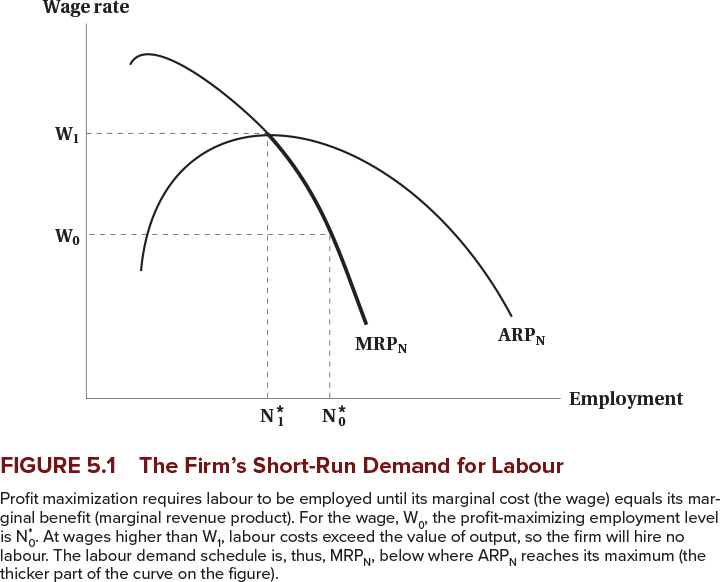
\includegraphics[width=0.71\linewidth]{ben54842_0501}.
\end{frame}

\begin{frame}{Shutdown Region and Curve Segment}
\transfade
\begin{itemize}[<+->]
  \item Shut down if the wage exceeds the \textbf{average revenue product} of labour.
  \item Short-run labour demand coincides with \(\text{MRP}_N\) \textit{below} the \(ARP\)–\(MRP\) intersection.
  \item \textbf{Downward sloping:} Diminishing marginal returns; \(\downarrow w \Rightarrow \uparrow N\).
\end{itemize}
\end{frame}

% ============================================================
\section{Long-Run Labour Demand}
% ============================================================

\begin{frame}{Isoquants and Isocosts}
\transfade
\begin{itemize}[<+->]
  \item \textbf{Isoquant:} Combinations of \(K\) and \(N\) yielding a given \(Q\); diminishing MRTS.
  \begin{itemize}
  \item \textbf{MRTS }-- the rate at which a firm can substitute labor for capital while keeping production output constant
  \end{itemize}
  \item \textbf{Isocost:} \(TC=rK+wN\), all input bundles with the same cost.
\end{itemize}
\end{frame}

\begin{frame}{Figure 5.2: Isoquants, Isocost, and Cost Minimization}
\centering
\vspace{2em}

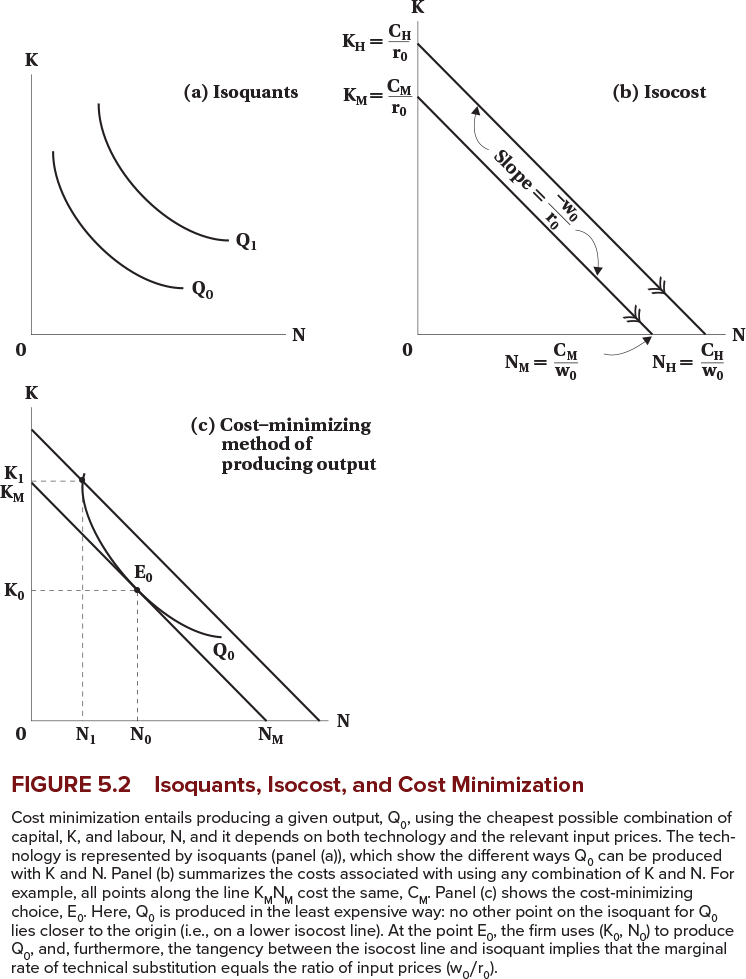
\includegraphics[width=0.44\linewidth]{ben54842_0502}.
\end{frame}


%------------------------------------------------

\begin{frame}{Panel (a): Isoquants}
\begin{itemize}[<+->]
\item Curves labeled $Q_0$ and $Q_1$ are \textbf{isoquants}
\item Each isoquant shows all $(K,N)$ combinations producing the same output
\item $Q_1$ represents a higher level of output than $Q_0$
\item Isoquants are:
\begin{itemize}[<+->]
\item Downward sloping (inputs are substitutes)
\item Convex to the origin (diminishing MRTS)
\end{itemize}
\end{itemize}
\end{frame}

%------------------------------------------------

\begin{frame}{Isoquants: Interpretation}
\begin{itemize}[<+->]
\item Moving \textbf{along} an isoquant:
\begin{itemize}[<+->]
\item Output remains fixed
\item Firm substitutes capital for labour or vice versa
\end{itemize}
\item Moving to a \textbf{higher isoquant} (from $Q_0$ to $Q_1$):
\begin{itemize}[<+->]
\item Requires more inputs
\item Represents an increase in output
\end{itemize}
\item Technological change (not shown):
\begin{itemize}[<+->]
\item Inward shift: productivity improvement
\item Outward shift: productivity decline
\end{itemize}
\end{itemize}
\end{frame}

%------------------------------------------------

\begin{frame}{Panel (b): Isocost Lines}
\begin{itemize}[<+->]
\item Isocosts show combinations of $K$ and $N$ with the same total cost
\item Total cost:
\[
C = w_0 N + r_0 K
\]
\item $w_0$: wage rate, $r_0$: rental rate of capital
\item Lines labeled $C_M$ and $C_H$ represent different cost levels
\end{itemize}
\end{frame}

%------------------------------------------------

\begin{frame}{Isocost Lines: Slopes and Intercepts}
\begin{itemize}[<+->]
\item Vertical intercepts:
\[
K_M = \frac{C_M}{r_0}, \qquad K_H = \frac{C_H}{r_0}
\]
\item Horizontal intercepts:
\[
N_M = \frac{C_M}{w_0}, \qquad N_H = \frac{C_H}{w_0}
\]
\item Slope of the isocost:
\[
\text{Slope} = -\frac{w_0}{r_0}
\]
\item Interpretation: trade-off between labour and capital holding cost fixed
\end{itemize}
\end{frame}

%------------------------------------------------

\begin{frame}{Shifts and Rotations of Isocosts}
\begin{itemize}[<+->]
\item Increase in total cost $C$:
\begin{itemize}[<+->]
\item Parallel outward shift of the isocost
\end{itemize}
\item Increase in wage $w_0$:
\begin{itemize}[<+->]
\item Isocost becomes steeper
\item Rotates inward around the $K$-intercept
\end{itemize}
\item Increase in rental rate $r_0$:
\begin{itemize}[<+->]
\item Isocost becomes flatter
\item Rotates inward around the $N$-intercept
\end{itemize}
\end{itemize}
\end{frame}

%------------------------------------------------

\begin{frame}{Panel (c): Cost-Minimizing Choice}
\begin{itemize}[<+->]
\item Firm wants to produce $Q_0$ at the lowest possible cost
\item Chooses point $E_0$ where:
\begin{itemize}[<+->]
\item Isoquant $Q_0$ is tangent to the lowest isocost
\end{itemize}
\item Optimal input bundle:
\[
(K_0, N_0)
\]
\item Any other point on $Q_0$ lies on a higher-cost isocost
\end{itemize}
\end{frame}

%------------------------------------------------

\begin{frame}{Tangency Condition at the Optimum}
\begin{itemize}[<+->]
\item At the cost-minimizing point $E_0$:
\[
MRTS_{N,K} = \frac{MPP_N}{MPP_K}
\]
\item Cost minimization requires:
\[
\frac{MPP_N}{MPP_K} = \frac{w_0}{r_0}
\]
\item Interpretation:
\begin{itemize}[<+->]
\item The rate at which the firm can trade $K$ for $N$ in production
\item Equals the rate at which the market allows substitution via prices
\end{itemize}
\end{itemize}
\end{frame}

%------------------------------------------------

\begin{frame}{Why Other Points Are Not Optimal}
\begin{itemize}[<+->]
\item Points like $(K_1, N_1)$:
\begin{itemize}[<+->]
\item Produce $Q_0$ but lie on higher isocosts
\item Are more expensive than $E_0$
\end{itemize}
\item Points closer to the origin but not tangent:
\begin{itemize}[<+->]
\item Either infeasible or violate cost minimization
\end{itemize}
\item Only tangency ensures minimum cost for given output
\end{itemize}
\end{frame}

%------------------------------------------------

\begin{frame}{Movements vs Shifts}
\begin{itemize}[<+->]
\item \textbf{Movement along an isoquant}:
\begin{itemize}[<+->]
\item Output fixed
\item Input mix changes
\item Driven by changes in relative prices
\end{itemize}
\item \textbf{Shift of isoquants}:
\begin{itemize}[<+->]
\item Caused by technological change
\item Affects productivity and labour demand
\end{itemize}
\item \textbf{Rotation of isocosts}:
\begin{itemize}[<+->]
\item Caused by changes in $w_0$ or $r_0$
\item Drives substitution between labour and capital
\end{itemize}
\end{itemize}
\end{frame}












\begin{frame}{Figure 5.3: Deriving the Labour Demand Schedule }
\centering
\vspace{2em}

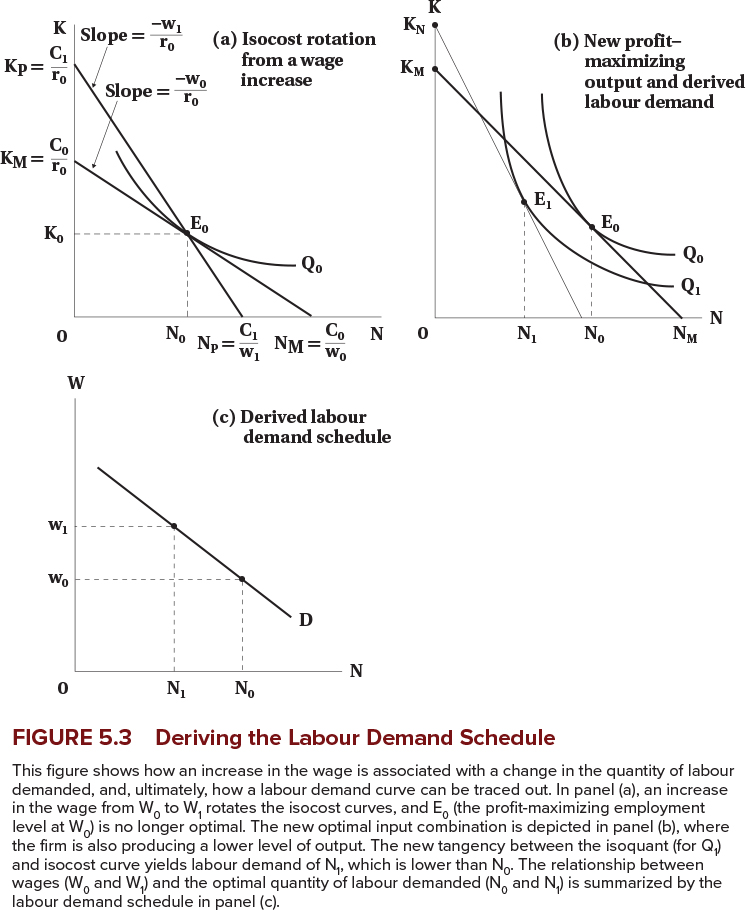
\includegraphics[width=0.46\linewidth]{ben54842_0503}.
\end{frame}

\begin{frame}{Cost Increases Under Perfect Competition}
\transfade
\begin{itemize}[<+->]
  \item Higher \(w\) rotates the isocost inward; substitute \(K\) for \(N\).
  \item Firm MC and AC shift up; industry output falls and price rises.
\end{itemize}
\end{frame}

\begin{frame}{Monopoly Case: Cost Increases}
\transfade
\begin{itemize}[<+->]
  \item Monopolist: \(MR=MC\), price setter, \(P>MC\).
  \item Hiring more labour lowers both MPP and MR; output and employment responses differ from competition.
\end{itemize}
\end{frame}

\begin{frame}{Figure 5.4: The Effect of a Cost Increase on Output }
\centering
\vspace{2em}

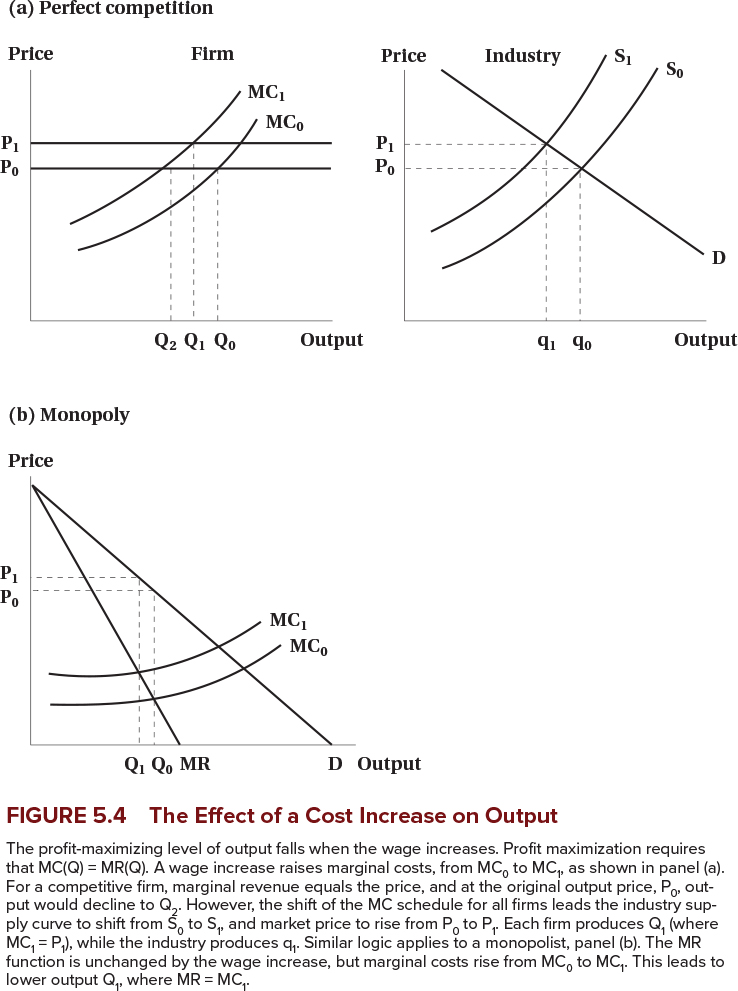
\includegraphics[width=0.41\linewidth]{ben54842_0504}.
\end{frame}

\begin{frame}{Substitution vs.\ Scale Effects}
\transfade
\begin{itemize}[<+->]
  \item \textbf{Substitution effect:} Use cheaper inputs instead of labour.
  \item \textbf{Scale effect:} Higher costs shrink output scale, reducing all inputs.
\end{itemize}
\end{frame}

\begin{frame}{Figure 5.5: Substitution and Scale Effects of a Wage Change }
\centering
\vspace{2em}

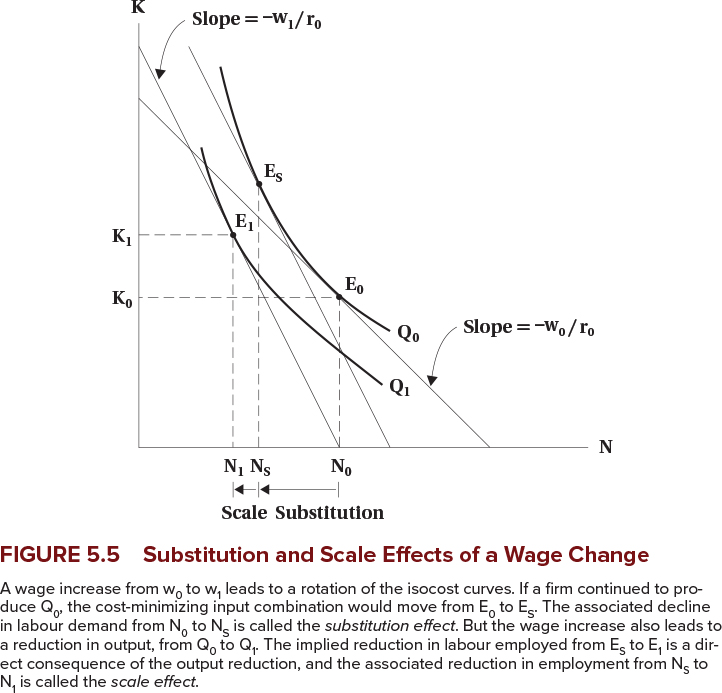
\includegraphics[width=0.61\linewidth]{ben54842_0505}.
\end{frame}

% ============================================================
\section{Worked Examples: Offshoring}
% ============================================================

\begin{frame}{Worked Example: Offshoring (Toy Inc.)}
\transfade
\small
Toy Inc.\ can hire assembly workers in Canada or abroad; workers are \textbf{close substitutes}. Outsourcing abroad \(\Rightarrow\) lower effective wage for that task \(\Rightarrow\) \textbf{reduces Canadian employment}.
\end{frame}

\begin{frame}{Toy Inc. }
\centering
\vspace{2em}

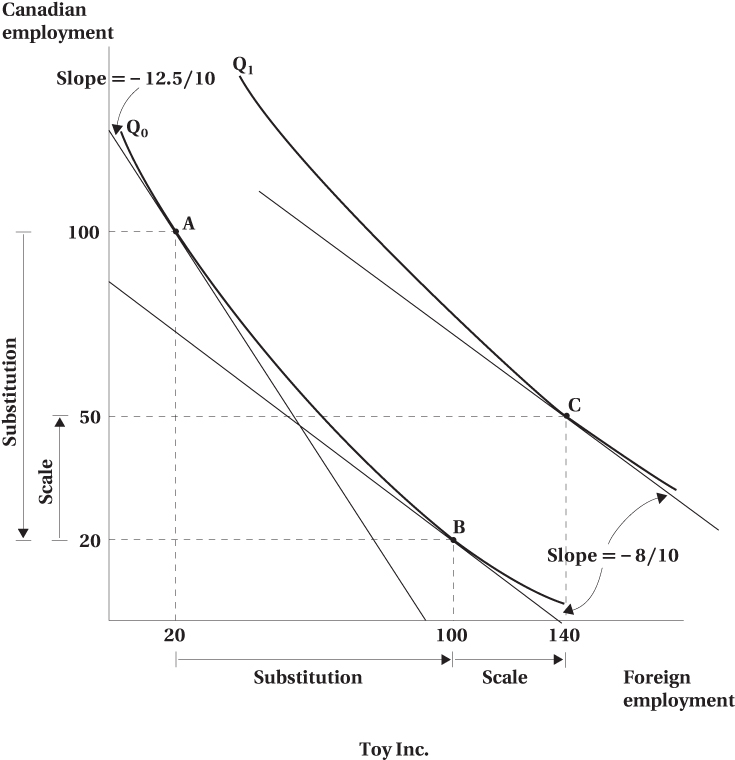
\includegraphics[width=0.5\linewidth]{ben54842_un0501}.
\end{frame}

\begin{frame}{Worked Example: Offshoring (Bridge Inc.)}
\transfade
\small
Bridge Inc.\ builds bridges; Canadian engineers/designers/managers work at home; construction workers hired abroad. Inputs are \textbf{complements}. Outsourcing on-site construction \textbf{does not reduce} Canadian employment of complementary skilled workers.
\end{frame}

\begin{frame}{Bridge Inc. — Illustration }
\centering
\vspace{2em}

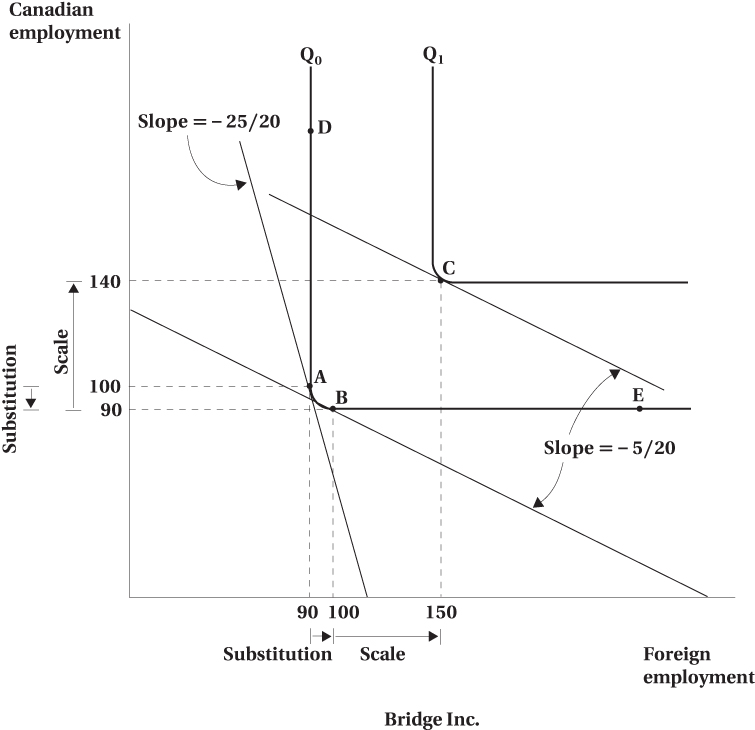
\includegraphics[width=0.5\linewidth]{ben54842_un0502}.
\end{frame}

% ============================================================
\section{Short vs.\ Long Run}
% ============================================================

\begin{frame}{Linking Horizons}
\transfade
\begin{itemize}[<+->]
  \item \textbf{Short run:} \(K\) fixed; no substitution effect.
  \item \textbf{Long run:} \(K\) variable; substitution \(\Rightarrow\) larger employment response to wage changes.
\end{itemize}
\end{frame}

\begin{frame}{Figure 5.6: Labour Demand in Short vs.\ Long Run}
\centering
\vspace{2em}

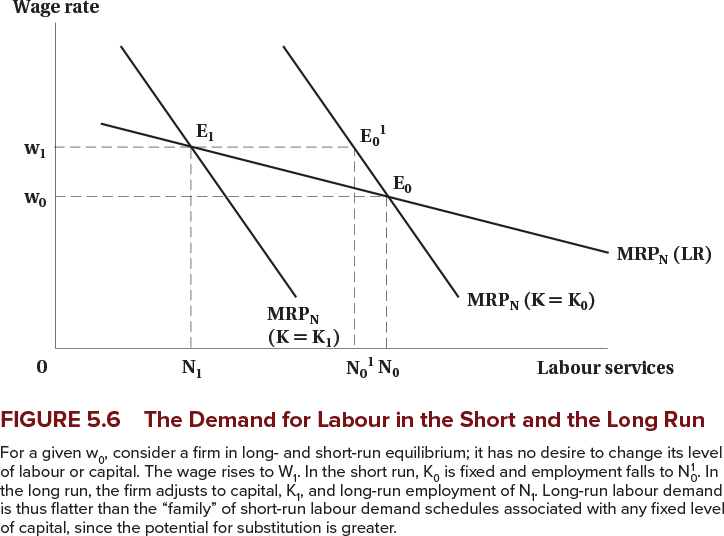
\includegraphics[width=0.79\linewidth]{ben54842_0506}.
\end{frame}

\begin{frame}{Cost Minimization in Public/Quasi-Public Sectors}
\transfade
Organizations target \textbf{given output at minimum cost}. Scale vs.\ substitution effects remain key to labour demand responses.
\end{frame}

% ============================================================
\section{Elasticity of Labour Demand}
% ============================================================

\begin{frame}{Definition and Measurement}
\transfade
\begin{itemize}[<+->]
  \item Demand for labour typically falls when wages rise.
  \item Elasticity \( \varepsilon_{N,w} = \frac{\%\ \Delta N}{\%\ \Delta w} \).
\end{itemize}
\end{frame}

\begin{frame}{Figure 5.7: Inelastic vs.\ Elastic Labour Demand }
\centering
\vspace{2em}

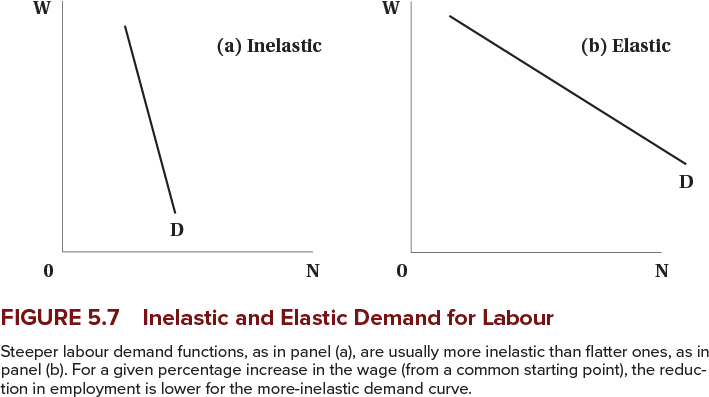
\includegraphics[width=1.03\linewidth]{ben54842_0507}.
\end{frame}

\begin{frame}{Determinants of Elasticity}
\transfade
\begin{itemize}[<+->]
  \item Availability of \textbf{substitute inputs}.
  \item Supply conditions of substitute inputs.
  \item Elasticity of demand for \textbf{output}.
  \item Ratio of \textbf{labour cost} to \textbf{total cost}.
\end{itemize}
\end{frame}

\begin{frame}{Implications}
\transfade
\begin{itemize}[<+->]
  \item Poor substitutability \(\Rightarrow\) inelastic labour demand.
  \item Inelastic product demand \(\Rightarrow\) inelastic labour demand.
  \item Small labour-cost share \(\Rightarrow\) inelastic labour demand.
\end{itemize}
\end{frame}

% ============================================================
\section{Globalization, Trade, and ICT}
% ============================================================

\begin{frame}{Changing Demand Conditions}
\transfade
\begin{itemize}[<+->]
  \item TPP and other trade agreements.
  \item Offshoring and ICT diffusion.
  \item Media narratives vs.\ measured employment impacts.
\end{itemize}
\end{frame}

\begin{frame}{The Impact of Trade in a Single Labour Market}
\transfade
\begin{itemize}[<+->]
  \item Production does not automatically move to lower-wage countries.
  \item Profit-maximization depends on \textbf{both} costs and productivity.
  \item Foreign and Canadian labour may be \textbf{imperfect substitutes}.
\end{itemize}
\end{frame}

\begin{frame}{TABLE 5.1: Productivity (2000) and Changes in Productivity, Hourly Compensation, and Unit Labour Costs, 2000--2018}
\transfade
\scriptsize
\begin{tabular}{lcccc}
\toprule
\textbf{Country} & \textbf{Productivity in 2000 (as \% of Canada)} & \textbf{\% Change in Productivity} & \textbf{\% Change in Compensation} & \textbf{\% Change in Unit Labour Costs} \\
\midrule
Korea & 45 & 99 & 32 & --23 \\
Mexico & 46 & 2 & --44 &  \\
New Zealand & 79 & 21 & 76 & 42 \\
Japan & 87 & 20 & --38 & --48 \\
Australia & 99 & 24 & 45 & 22 \\
Canada & 100 & 18 & 16 & 1 \\
Spain & 102 & 17 & 18 & --1 \\
United Kingdom & 111 & 18 & --5 & --18 \\
Finland & 116 & 20 & 24 & 5 \\
Italy & 119 & 1 & 14 & 13 \\
Sweden & 121 & 28 & 17 & --7 \\
United States & 123 & 30 & 2 & --19 \\
Germany & 126 & 19 & 9 & --6 \\
France & 129 & 18 & 19 & 6 \\
Netherlands & 135 & 15 & 19 & 3 \\
Denmark & 135 & 22 & 33 & 10 \\
Switzerland & 136 & 19 & 40 & 19 \\
Belgium & 143 & 14 & 21 & 5 \\
Norway & 164 & 16 & 46 & 27 \\
\textbf{Average} & \textbf{111} & \textbf{22} & \textbf{18} & \textbf{2} \\
\bottomrule
\end{tabular}
\end{frame}

\begin{frame}{Figure 5.8: Relative Trends in Labour Costs and Productivity (Canada vs.\ U.S.) }
\centering
\vspace{2em}

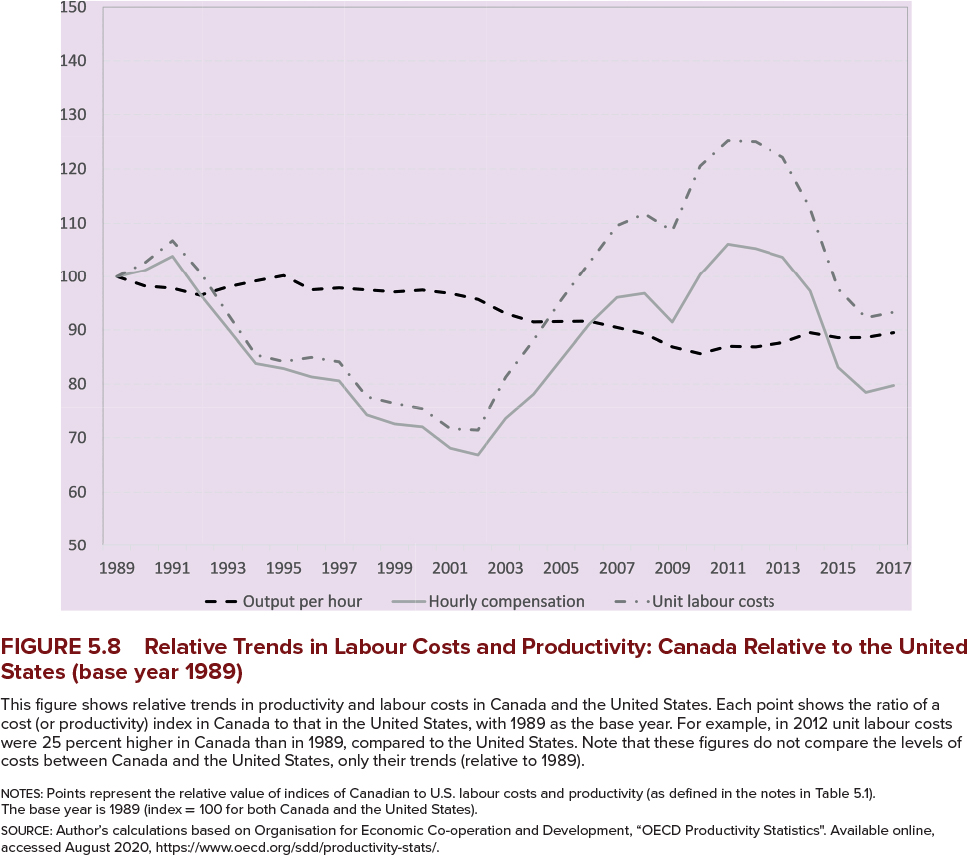
\includegraphics[width=0.63\linewidth]{ben54842_0508}.
\end{frame}

\begin{frame}{Figure 5.9: Trade, Consumption, and Production in a Simple Economy }
\centering
\vspace{2em}

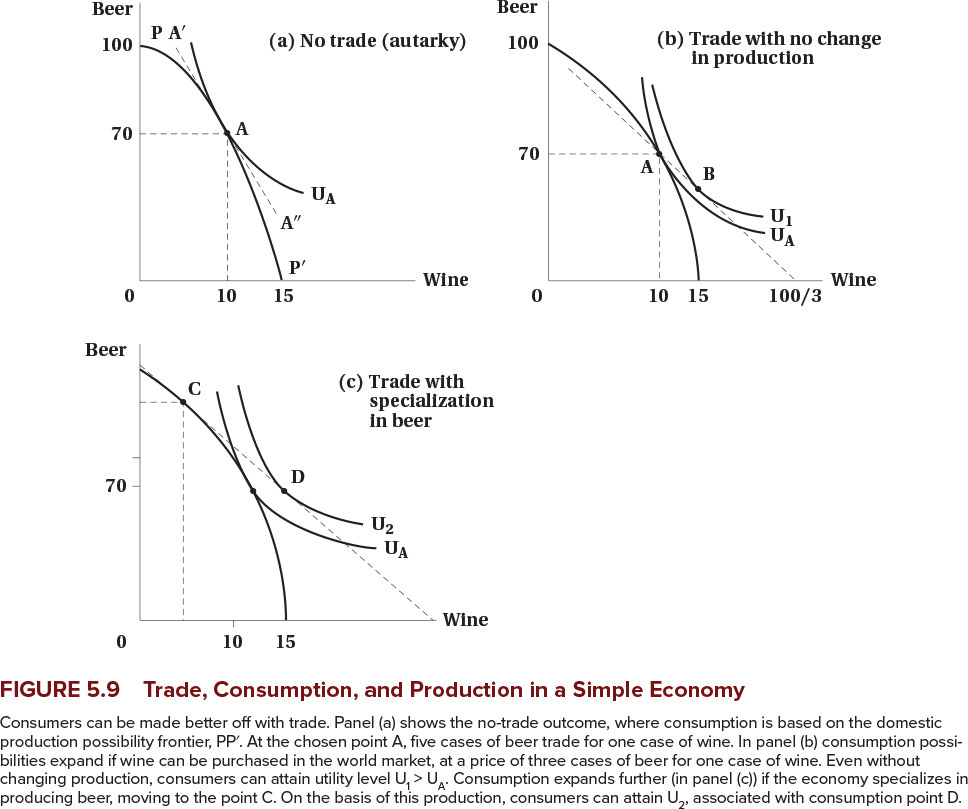
\includegraphics[width=0.64\linewidth]{ben54842_0509}.
\end{frame}

\begin{frame}{Evidence: CUFTA/NAFTA \& Offshoring}
\transfade
\begin{itemize}[<+->]
  \item Short-run adjustment costs existed.
  \item Long-run benefits of FTA were significant.
  \item Measured impacts of offshoring on employment have been modest.
\end{itemize}
\end{frame}

\begin{frame}{Other Demand-Side Factors}
\transfade
\begin{itemize}[<+->]
  \item “Declining middle” and wage polarization.
  \item Shift from “smokestack” to flexible, modular production.
  \item ICT reshaped internal firm organization and business practices.
\end{itemize}
\end{frame}


\begin{frame}{Summary}
\transfade
\begin{itemize}[<+->]
  \item \textbf{Derived demand:} Labour demand stems from product demand.
  \item \textbf{Short run:} Hire to \( \text{MRP}=w \).
  \item \textbf{Long run:} Substitution and scale effects; demand more elastic.
  \item \textbf{Elasticity drivers:} Substitutability, output demand elasticity, labour-cost share.
  \item \textbf{Globalization/ICT:} Channels run via productivity, costs, and task (substitute vs.\ complement).
\end{itemize}
\end{frame}

% ============================================================
\begin{frame}
\centering
\Huge{\textbf{Thank You!}} \\

\end{frame}

\end{document}
